\documentclass[12pt,a4paper]{book}

\usepackage[utf8]{inputenc}
\usepackage[T1]{fontenc}
\usepackage{lmodern}

\usepackage{hyperref}
\usepackage{graphicx}
\usepackage[english, frenchb]{babel}

\usepackage{menukeys}

\usepackage{listings}	
\lstdefinestyle{customstyle}{
    basicstyle=\footnotesize,
    breakatwhitespace=false,         
    breaklines=true,                 
    captionpos=b,                    
    keepspaces=true,                                                                                       
    tabsize=4,
    frame=single %lines
}
 
\lstset{style=customstyle}	
	
\title{ArchPi cheat book}
\author{Jérémy Bardon}
				
\begin{document}
\frontmatter
	\maketitle
	\tableofcontents	

\mainmatter

\chapter*{Preface}
Howto book to learn you a few things you need to know about 
\href{http://archlinuxarm.org/platforms/armv6/raspberry-pi}{ArchLinux ARM} 
on \href{http://www.raspberrypi.org/help/what-is-a-raspberry-pi/}{RPi}. 
From basic setup of the system to side packages installation to turn 
your Raspberry into a music sharing or even a versioning control server.

\section*{Structure of book}
The first part of this book will be focused on system setup and 
basic settings as keyboard language, user account and others. 
The second part will describe how to install some third party sofwares 
as git and mpd server.

\section*{Author words}
I am not an expert in linux system as ArchLinux and even less in electronic 
stuff. However, as a developer I like to tinker with my new toy which is 
a Raspberry Pi. 

I had a lot of troubles when I decided to find uses for it 
and tried to install some third party software. As a result, I am glad to 
write this \og{}book\fg{} to help you to install things on your RPi with ArchLinux.

\chapter{Introduction}
	\section{Are you interested?}
This book is written by a non-specialist of ArchLinux with basic knowledge of 
linux system so I will try to made it as simple as possible for people 
who have no idea about what is console. Indeed, all commands will be 
explained for a better comprehension and an index will be available for you.
\\\\
No matter if you are an expert or a novice, you will be able to find 
how to install stuff on your your Pi plus tips which includes all the problems 
I encounter during my first installation.

	\section{What is a Raspberry Pi}
If you succeed to find this book I guess you allready know but some people 
buy a Raspberry with OpenELEC\footnote{Tiny linux system based on XBMC media center. 
More details on \href{http://openelec.tv}{openelec.tv}} pre-installed so here 
is a little explaination.
\\\\
The Raspberry Pi is a credit-size computer with low performances if you
compare with a common PC. Nevertheless, it means its power consumption is
very low (1W for B+ version\footnote{Most robust version of RPi with 512MB 
of RAM and 4 usb ports}) so it is not a problem to let it on forever. 
\newpage
\begin{figure}[h]
	\centering
	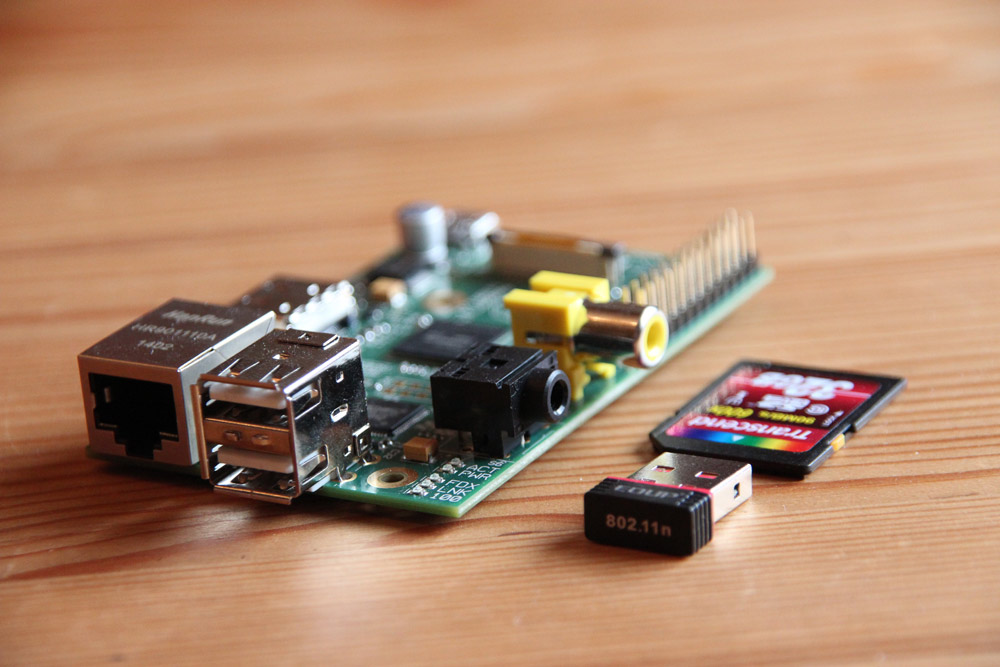
\includegraphics[scale=0.2]{images/RaspberrySize.jpg}
	\caption{Raspberry Pi B+}
	\label{figure:RaspberrySize}
\end{figure}

Finally if you install a good linux distribution on it you can turn this old computer
into a cheap server on which you will have the control. You can use it 
at home for file sharing, media player or others but it is also possible
to host a website which will be available on the internet\footnote{An example
of website hosted by a Rpi on \href{http://raspberrypi.goddess-gate.com}
{raspberrypi.goddess-gate.com}}.

	\section{ArchLinux versus \href{http://www.raspbian.org}{Raspbian}}
	\label{section:ArchVsRaspbian}
The operating system recommended by the Raspberry fundation is Raspbian -- a custom version of the famous Debian\footnote{One of the most popular linux 
system. See \href{https://www.debian.org/intro/about}{debian.org} for more details} system -- optimized for RPi hardware. 
\\\\
In general it will be the default choice for an inexperienced user to get
a user interface and most common softwares allready installed at the first boot.
However we forget the limited performances of the Raspberry and you will be able to realize that for yourself if you decided to install Raspbian. 
\\\\
A server does not need a user interface except a terminal which is enough 
to manage it everyday from anywhere. As a result, my choice has been focused 
on ArchLinux which is a pretty light and fast system. In addition, system 
updates are based on rolling release \footnote{Definition on \href{http://
en.wikipedia.org/wiki/Rolling\_release}{wikipedia/Rolling\_release}} model, 
so it means you do not have one version of the system. You will just receive 
updates frequentely -- as soon as their availability -- and it will be not 
necessary to reboot during the upgrade process.

%\documentclass[12pt,a4paper]{book}\usepackage{hyperref}\usepackage[english, frenchb]{babel}\begin{document}
\chapter{ArchLinux installation}
\section{We are \textsc{Noobs}}
There are two ways to install ArchLinux on a Raspberry Pi: the first is 
the ArchLinux way -- no idea if it is the same with other systems -- and 
the second is an official manager which works with many systems.

\begin{itemize}
	\item follow instructions from archlinuxarm.org\footnote{Specific 
		  instruction on \href{http://archlinuxarm.org/platforms/armv6/
		  raspberry-pi}{archlinuxarm.org/platforms/armv6/raspberry-pi}} but 
		  you need to have a linux system
		  
	\item use \textsc{Noobs}, an operating system install manager provided by 
		  the Raspberry fundation\footnote{Details on \href{http://
		  www.raspberrypi.org/help/noobs-setup}{www.raspberrypi.org/help/
		  noobs-setup}}\\
\end{itemize}

I choose \textsc{Noobs} because it is the easiest way to install a
system on a RPi and in addition you get an extra \og{}boot manager\fg{} which 
is usefull. Moreover, you can complete the full setup of your SD card on any 
system by following the RPi website guide.
\\\\
\textsc{Noobs} is available on two forms: one for offline installation 
and the other -- the smallest one -- downloads automatically the last release 
of the system online. The offline installer contains many systems -- which 
takes a large space -- but you can just keep ArchLinux and remove others 
(in \texttt{os} folder). Anyway, you need to know that other systems files 
will be keeped after the installation so it is loose space. If you still want 
to use the offline way because you have no choices, you will have to find  
an older version of \textsc{Noobs} because ArchLinux has been removed since  
the last release.

\section{Installer usage}
% wifi ou ethernet

%\end{document}

%\documentclass[12pt,a4paper]{book}\usepackage[utf8]{inputenc}\usepackage[T1]{fontenc}\usepackage{lmodern}\usepackage{hyperref}\usepackage{graphicx}\usepackage[english, frenchb]{babel}\usepackage{listings}	\lstdefinestyle{customstyle}{basicstyle=\footnotesize,breakatwhitespace=false,breaklines=true,captionpos=b,keepspaces=true,tabsize=4,frame=single}\lstset{style=customstyle}\usepackage{menukeys}\begin{document}
\chapter{Basic setup}

\section{Change language}
There are no default languages selected in ArchLinux but the keyboard map is set to 
qwerty\footnote{Most common layout for keyboards} at the beginning. To choose 
your language you have to complete two steps and then the system will be able to 
use it for characters encoding and some softwares as \texttt{nano}.

\subsection{Enable yours}
Before choosing yours it is necessary to enable it in \texttt{/etc/locale.gen}
file with \texttt{locale} tools. 

You will need to use \texttt{nano} to edit the configuration file -- \keys{\ctrl 
+ W} can help you to search -- and remove \og\#\fg{} before the language you want 
to enable (fr\_FR.UTF-8 for example), to save your changes press \keys{\ctrl + X}.
\\
\begin{lstlisting}[language=bash,caption=Enable your language]
$ locale # Current language settings

# Edit the /etc/locale.gen file
$ nano /etc/locale.gen

$ locale-gen # Update available languages
$ locale -a  # See available languages
\end{lstlisting}

\subsection{Change your settings}
The second step is to set the language and configure your keyboard map. 
Notice that you will have to logout for the system to take into account 
changes you made with language setup.
\\ 
\begin{lstlisting}[language=bash,caption=Change language settings]
$ localectl status
  System Locale: n/a  # System language
      VC Keymap: n/a  # Virtual console
     X11 Layout: n/a  # Graphic interface
     
# Change system language (enabled one)
$ localectl set-locale LANG=fr_FR.UTF-8

# List of keymaps, choose the one you want "fr-pc" for example
$ localectl list-keymaps

# Change settings 
# no-convert not update VC with X11 and vice versa
$ localectl set-keymap --no-convert fr-pc     # VC Keymap
$ localectl set-x11-keymap --no-convert fr-pc # X11 Layout

# Logout to apply changes
$ exit
\end{lstlisting}

\section{Configure wifi connexion}
\subsection{Check your dongle}
The first thing you can do is check if your dongle has been recognized by 
the system and can be used.

\begin{lstlisting}[language=bash,caption=Check wifi device]
$ ifconfig -a wlan # All wireless interfaces (also disabled)

# If you see a line with "wlan0" try to enable it
$ ip link set wlan0 up

# If you see again "wlan0" your dongle is working
# Disable it after the check
$ ifconfig wlan # Without -a show only enabled interfaces
$ ip link set wlan0 down
\end{lstlisting}

There are a lot of ways to connect your RPi to a network using a wifi dongle 
but all of them requires to install a package before -- wifi-menu needs 
dialog, iw and wpa\_supplicant are not installed -- so it is necessary to 
use an ethernet wire to begin.

\begin{lstlisting}[language=bash,caption=Install wireless dependencies]
# pacman is the package manager in ArchLinux
#        -S install a new package 
#
# dialog to get wifi-menu interface
# wpa_supplicant for wireless network protected with wpa keys
#
$ pacman -S dialog wpa_supplicant
\end{lstlisting}

\subsection{Searching the internet}
Once you installed all the packages -- synonym for software -- that wifi-menu 
needed to run you can launch it with \og{}\texttt{wifi-menu}\fg{} command.

\begin{figure}[h]
	\centering
	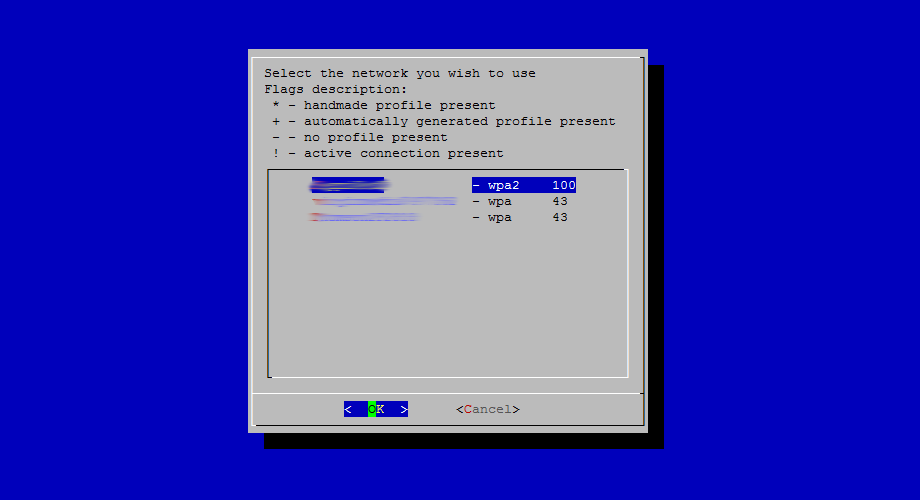
\includegraphics[scale=0.3]{images/WifiMenu.png}
	\caption{wifi-menu interface}
	\label{figure:WifiMenu}
\end{figure}

Then, select your network -- with \keys{\arrowkeyup} and \keys{\arrowkeydown} -- 
, type your password (if required) and you will be connected to your wireless 
network.
\newpage
\section{Create yourself}
\subsection{Simple user}
The default username and password for ArchLinux are \texttt{root/root}, this 
user got all right on the system it means he can do anything -- even break 
the system -- so it is not recommanded to use it.
\\
\begin{lstlisting}[language=bash,caption=Create a new user called jeremy]
$ useradd -m jeremy # Creates user jeremy and his home folder
$ passwd jeremy     # Changes jeremy password
\end{lstlisting}

Now we have a new user account for everydays usage. You can see all users on 
your system with \og{}\texttt{cat /etc/passwd}\fg{} which will display the 
content of the config file for users.

\subsection{Very important user}
It is possible to specify user rights with \texttt{visudo} command, the general syntax for one user is 
the following \og{}\texttt{username machine=(targetuser) commands}\fg{}, 
let's look at some details:


%# Attribute rights with a specific format
%$ visudo
%# Add new line: "jeremy ALL=(ALL) ALL"

\begin{description}
\item[username] name you gave to \texttt{useradd} command
\item[machine] machine on where rights are applied, ALL in general
\item[target user] user that we takes the rights
\item[command] allowed commands separated with one coma -- no spaces --, 
use exclamation mark for banned commands
\end{description}

%\end{document}


\end{document}
